% started 18Nov2018
% finished 20Nov2018
\documentclass[10pt]{article}
\setlength\parindent{0pt}
\usepackage{colortbl}
\usepackage{cool}
\usepackage[utf8]{inputenc}
\usepackage[T1]{fontenc}
\usepackage{graphicx}
\usepackage{subfig}
\usepackage{wrapfig}
\usepackage{color}
\usepackage{amsmath}
\usepackage{amssymb}
\usepackage{nicefrac} 
\usepackage{listings}
\usepackage{geometry}
\geometry{a4paper}
\usepackage{float}
\usepackage[bottom]{footmisc}			%to make footnotes stick to the page bottom
\usepackage[nottoc,numbib]{tocbibind}	%to make bibliography appear in Contents
\floatstyle{boxed} 
\linespread{1}							%to change space between lins {1} is default
\usepackage[round, sort&compress, comma, authoryear]{natbib}
\usepackage{hyperref} 
\usepackage{tcolorbox}

\DeclareMathOperator{\sign}{\mathbf{sgn}    }
\DeclareMathOperator{\payoff}{\mathbf{Payoff}    }

\title{Modelling Implied Volatility: Neural Network Method }
\author{YASHKIR CONSULTING \quad www.yashkir.com}
\date{\today}
\usepackage[toc,page]{appendix}
\begin{document}
\maketitle
\tableofcontents	

\section{Introduction}

Implied volatility surface \citep{hjm} is used for pricing vanilla options given price/strike ratio and time to maturity;

\section{The problem formulation}\label{hjm}
Given historical data (option price, spot price, strike price, time to maturity) for certain period of time, to build a model for implied volatility as function of spot/strike ratio $\kappa$ and time to maturity $T$. File with historical data in general case can be formatted as follows:
\begin{table}[H] 
\title{Input data file: \\} 
\label{indata}
\begin{tabular}{ |llllllllll|}
\hline
$x_{00}$ & $\cdots$  & $x_{0j}$ & $\cdots$  & $x_{0,J-1}$ & $y_{00} $ & $\cdots$ & $y_{0i}$ & $\cdots$ &$y_{0,I-1}$ \\
$\cdots$ & $\cdots$ & $\cdots$ & $\cdots$& $\cdots$& $\cdots$& $\cdots$& $\cdots$& $\cdots$& $\cdots$ \\
$x_{n0}$ & $\cdots$  & $x_{nj}$ & $\cdots$ & $x_{n,J-1}$ & $y_{n0} $ & $\cdots$ & $y_{ni}$ & $\cdots$ &$y_{n,I-1} $ \\
$\cdots$ & $\cdots$ & $\cdots$ & $\cdots$& $\cdots$& $\cdots$& $\cdots$& $\cdots$& $\cdots$& $\cdots$ \\
$x_{N-1,0}$ & $\cdots$  & $x_{N-1,j}$ & $\cdots$ & $x_{N-1,J-1}$ & $y_{N-1,0} $ & $\cdots$ & $y_{N-1,i}$ & $\cdots$ &$y_{N-1,I-1}  $ \\
\hline
\end{tabular}
\end{table}

In this file the number of samples is $N$, the number of input variables is $J$, the number of output values is  $I$.
To build a model we will use deep (with the number of layers $L$) neural network structure. The first (input) layer has $J$ nodes, hidden layers may have different number of nodes, but we'll assume that the number of nodes in all layers is the same $J$, except in output layer with $I$ nodes.
 
The index $n$ indicates a sample, parameters $\vec x_n$ contain the spot price/strike ratio, time-to-maturity, and some more. Values $\vec y_n$ contain historical implied volatilities, and may have some other variables. 

The propagation of the input signal $x_{nj}$ (or $\textbf{x}$) is as follows:
\begin{enumerate}
\item Nodes of the input layer ($l=0$) "emit" values $a_{n0j} \equiv x_{nj} $
\item Layer $l$ ($l=1\cdots L-1$): \\
Output signals from nodes (neurons) of the layer $(l-1)$ are combined as biased weighted average values for inputs into nodes $j$ of the layer $l$
 \begin{equation}
 \label{zab}
z_{nlj} = \sum_{k=0}^{J-1} a_{n,l-1,k}w_{lkj} + b_{lj}
\end{equation}
(Note: within sample $n$ the vector/matrix form would be $\vec{z}_n^l = \vec{a}_n^{l-1}\textbf{w}_l + \vec {b}_l$. 
Weight matrices $\textbf{w}_l$ and biases $\vec {b}_l$ will be found as a result of the neural network iterative "training".)\\
The output of the $j^{th}$-neuron of the layer $l$ is emitted as nonlinear transformation of  $\vec{z}_n^l $ 
\begin{equation}
\label{a_out}
a_{nlj} = \sigma(z_{nlj})
\end{equation}
where function $\sigma()$ is, for example, a sigmoid function:
\begin{equation}
\sigma(x) = \frac{1}{1+ e^{-x}}
\end{equation}
\item Output layer ($L-1$): \ldots \\
As the result of the propagation of the input signal $x_{nj}$ through neural network we have $a_{n,L-1,i}$ ($i=0 \cdots , I-1$), see the equation (\ref{a_out}). 

The modelling error for all samples is defined as:
\begin{equation}
\label{err}
E = \frac{1}{2}\sum_n \sum_{i=0}^{I-1} (a_{n,L-1,i} - y_{ni})^2
\end{equation}
\end{enumerate} 

The problem, therefor, can be formulated as follows: \\

\begin{tcolorbox}
To find neural network parameters (weight matrices $\textbf{w}_l$ and biases $\vec {b}_l$) by minimizing the error function $E$ (\ref{err}).
\end{tcolorbox}

\section{Minimization of the error function}
The minimum of the error function can be found using gradient descent algorithm for which partial derivatives of (\ref{err}) by components of  $\textbf{w}_l$ and $\vec {b}_l$ must be calculated using backpropagation procedure.
\subsection{Backpropagation}
\begin{enumerate}
\item Output layer ($L-1$). \\
Derivatives by weighted averages $z_{n,j,L-1}$
\begin{align}
\delta_{n,j,L-1} = \frac{\partial E}{\partial z_{n,j,L-1}} &= \frac{\partial E}{\partial a_{n,j,L-1}} \cdot \frac{\partial a_{n,j,L-1}}{\partial z_{n,j,L-1}} 
=  \frac{\partial E}{\partial a_{n,j,L-1}} \cdot \frac{\partial \sigma(z_{n,j,L-1})}{\partial z_{n,j,L-1}} \\
\text{where}\\
\frac{\partial E}{\partial a_{n,j,L-1}} &= \frac{\partial }{\partial a_{n,j,L-1}} 
\left[ \frac{1}{2}\sum_k \left( a_{n,k,L-1} - y_{nk}  \right)^2    \right] = a_{n,j,L-1} - y_{nj}\\
\frac{\partial \sigma(z_{n,j,L-1})}{\partial z_{n,j,L-1}} &\equiv \sigma^{'}(z_{n,j,L-1})  
\end{align} 

\item Hidden layers ($l=L-2,\cdots,1$); backpropagation:
\begin{align}
\delta_{n,j,l} &= \frac{\partial E}{\partial z_{njl}} = \sum_k \frac{\partial E}{\partial z_{n,k,l+1}} \frac{\partial z_{n,k,l+1}}{\partial z_{n,j,l}} = \sum_k \delta_{n,k,l+1} \frac{\partial }{\partial z_{njl}} \left( \sum_i a_{nil} w_{i,k,l+1}+b_{k,l+1} \right) \\
&=\sum_k \delta_{n,k,l+1} \frac{\partial }{\partial z_{njl}} \left( \sum_i \sigma(z_{nil}) w_{i,k,l+1}+b_{k,l+1} \right)=\sum_k \delta_{n,k,l+1} w_{j,k,l+1} \sigma^{'}(z_{njl})
\end{align}
\item Derivatives by bias variables $\vec {b}_l \quad (l=L-1, \ldots 1)$:
\begin{align}
&\frac{\partial E}{\partial b_{jl}}=\frac{\partial E}{\partial a_{njl}} \frac{\partial a_{njl}}{\partial z_{njl}}\frac{\partial z_{njl}}{\partial b_{jl}}=\delta_{njl} \quad\text{(for a single sample n)} \\
\beta_{jl}&=\frac{1}{N}\sum_{n=0}^{N-1}\delta_{njl} \quad\text{(averaged over all samples)}
\end{align}
\item Derivatives by weight matrix components:
\begin{align}
&\text{Partial derivative within n-th sample:}\\
\label{der_n}
&\frac{\partial E}{\partial w_{kjl}} =\frac{\partial E}{\partial z_{njl}} \frac{\partial z_{njl}}{\partial w_{kjl}}
=\delta_{njl}\frac{\partial }{\partial w_{kjl}} \left(  \sum_i a_{n,i,l-1}+b_{jl}  \right)=\delta_{njl}a_{n,k,l-1} \\
&\text{Derivative (\ref{der_n}) averaged over all samples:}\\
\label{der_N}
v_{kjl} &= \frac{1}{N}\sum_{n=0}^{N-1} \delta_{njl}a_{n,k,l-1} 
\end{align}
\item Gradient descent step:
\begin{align}
 w_{kjl}&= w_{kjl} - h \cdot v_{kjl} \\
 b_{jl} &= b_{jl} - h \cdot \beta_{jl}
\end{align}
Where $h$ is the iteration step (learning rate)
\end{enumerate}

\subsection{Neural Network Iteration (Learning) Algorithm}

\begin{equation}
\frac{dB(t,T)}{B(t,T)}=r(t)dt+\sum\limits_{p=0}^{2} \sigma_p(t,T)dW_p (t)
\end{equation} 
where $T$ is the bond maturity, $\sigma_p$ represents the bond price volatility of the stochastic driver number $p$, and $\vec {dW}(t)$ is a 3-tier Wiener process.
\subsection{Bond prices expressed through the stochastic integral}
Let $G(B)= \ln B$ and use the Ito's lemma \citep{ito} as follows
\begin{equation}
\label{ito}
dG = \frac{\partial G}{\partial B} dB + \frac{1}{2}\pderiv[2]{G}{B} (dB)^2
\end{equation}

\begin{multline}
\label{ito_calc}
d(\ln B) = \frac{1}{B} \left ( r \cdot B \cdot dt + \sum \limits_p \sigma_p B \cdot dW_p \right ) 
+ \frac{1}{2} \frac{1}{(-B^2)}\left ( r(t) B \cdot dt + \sum \limits_p \sigma_p B \cdot dW_p  \right )^2 \\
= r \cdot dt + \sum \limits_p \sigma_p \cdot dW_p  - \frac{1}{2}  \left ( r^2 \cdot (dt)^2 + 2r \cdot dt \sum \limits_p \sigma_p \cdot dW_p  + \sum \limits_{p,p^{'}} \sigma_p \sigma_{p'} \cdot dW_p \cdot dW_{p'} \right ) \\
= r \cdot dt +\sum \limits_p \sigma_p \cdot dW_p - \frac{1}{2}r^2 (dt)^2 - r \cdot dt \sum \limits_p \sigma_p \cdot dW_p - \frac{1}{2} \sum \limits_{p,p^{'}} \sigma_p \sigma_{p'} \cdot dW_p \cdot dW_{p'}
\end{multline}  
Note that processes $dW_p$ are correlated
\begin{equation}
\label{WWrho}
\langle  dW_p(t) dW_{p'}(t) \rangle = \rho_{pp'}dt
\end{equation}
Keeping in the  equation (\ref {ito_calc})  only terms with degree of  $dt$ equal or less than $ 1$ we arrive to the following equation for the process $ \ln B(t,T)$:

\begin{equation}
\label{dlnB}
d \ln B(t,T) = \left ( r(t) - \frac{1}{2} \sum \limits_{pp'}\sigma_p (t,T) \sigma_{p'} (t,T) \rho_{pp'} \right )dt+ \sum \limits_{p=0}^2 \sigma_p (t,T) dW_p (t,T)
\end{equation}

Integration of the equation (\ref{dlnB} from $s$ to $t$ leads to the integral expression of the bond price as a function of bond volatilities:
\begin{equation}
\label{logBtT}
 \ln B(t,T)- \ln B(s,T) = \int \limits_s^t \left ( r(q)  - \frac{1}{2}
\sum \limits_{pp'} \rho_{pp'} \sigma_{p}(q,T) \sigma_{p'} (q,T) \right )  dq +
 \int \limits_s^t \sum \limits_p \sigma_{p}(q,T) dW_p(q) 
\end{equation}
or 
\begin{equation}
\label{BB}
 \frac{B(t,T)}{B(s,T)}= e^ {\int \limits_s^t \left ( r(q)  - \frac{1}{2}
\sum \limits_{pp'} \rho_{ pp'} \sigma_{p}(q,T) \sigma_{p'} (q,T) \right )  dq +
 \int \limits_s^t \sum \limits_p \sigma_{p}(q,T) dW_p(q) }
\end{equation}

This equation can be further simplified as follows. The equation (\ref{BB}) with $T=t$ becomes:
\begin{equation}
\label{Btt}
 \frac{B(t,t)}{B(s,t)}= e^ {\int \limits_s^t \left ( r(q)  - \frac{1}{2}
\sum \limits_{pp'} \rho_{ pp'} \sigma_{p}(q,t) \sigma_{p'} (q,t) \right )  dq +
 \int \limits_s^t \sum \limits_p \sigma_{p}(q,t) dW_p(q) }
\end{equation}
Combining (\ref{BB}) and (\ref{Btt}) we find (note that $B(t,t)=1$):
\begin{equation}
\label{BBB}
 B(t,T) = \frac{B(s,T)}{B(s,t)} e^ {\left \{ - \frac{1}{2}
\sum \limits_{pp'} \rho_{ pp'} \int \limits_s^t  [ \sigma_{p}(q,T) \sigma_{p'} (q,T)  - \sigma_{p}(q,t) \sigma_{p'} (q,t) ]  dq +
 \int \limits_s^t \sum \limits_p (\sigma_{p}(q,T)- \sigma_{p}(q,t) ) dW_p(q) \right \}}
\end{equation}
In the last equation (\ref {BBB}) the bond price at time $t$ maturing at $T$ is expressed through correlation matrix $\hat {\rho}$, volatility functions $\sigma_p (t,T)$ and Wiener processes $dW_p(t)$.

\subsection{Bond price and instantenious forward rate}

The instantanious forward rate $f(t,u)$ is defined by the following expression

\begin{equation}
\label{Bef}
 B(t,T) = e^ { - \int \limits_t^T f(t,u) du }
\end{equation}
which is equivalent to 
\begin{equation}
\label{fB*}
 f(t,T) = \frac{\partial}{\partial t}   \ln B(t,T)
\end{equation}

The differential of $f(t,T)$ can be calculated using (\ref{fB*}) and ( \ref{dlnB}):

\begin{multline}
\label{df}
 df(t,T) = d \left ( \frac{\partial}{\partial t}   \ln B(t,T)    \right )= \frac{\partial}{\partial t} \left ( d \ln B(t,T)\right )= - \frac{\partial}{\partial T} \left ( d \ln B(t,T)\right ) \\
 = -\frac{\partial}{\partial T} \left [  r(t) \cdot dt - \frac{1}{2} \sum \limits_{pp'} \rho_{pp'} \sigma_p(t,T) \sigma_{p'} (t,T) dt  + \sum \limits_{p} \sigma_p (t,T)dW_p(t) \right ]
\end{multline}
The instantaneous forward rate volatility can be introduced as
\begin{equation}
\label{sdot}
\dot {\sigma}_p(t,T) = \frac{\partial}{\partial T}   \sigma_p (t,T)
\end{equation}
or
\begin{equation}
\label{sB}
\sigma_p (t,T) = \int \limits_t^T \dot {\sigma}_p(t,u) du   
\end{equation}
Substitution of $\sigma_p (t,T)$ in the equation (\ref{df}) with (\ref{sB})  leads to:
\begin{multline}
\label{dfsdot}
 df(t,T) = \frac{1}{2}\sum \limits_{pp'} \rho_{pp'} \left [ \frac{\partial {\sigma_p(t,T)}}{\partial T} \sigma_{p'}(t,T)+  \sigma_{p}(t,T)  \frac{\partial {\sigma_{p'}(t,T)}}{\partial T}  \right ]dt-\sum \limits_p \frac{\partial {\sigma_p(t,T)}}{\partial T} dW_p (t) \\
 = \sum \limits_{pp'} \rho_{pp'} \dot {\sigma}_p(t,T) \left ( \int \limits_t^T \dot {\sigma}_{p'}(t,u)du \right )dt-\sum \limits_p \dot {\sigma}_p(t,T)dW_p(t)
\end{multline}
Integrate (\ref{dfsdot}) by $t$ (from $s$ to $t$) and (for convenience) replace $T$ with $u$. We then have:
\begin{equation}
\label{ftu}
f(t,u) - f(s,u) =  \sum \limits_{pp'} \rho_{pp'} \int \limits_s^t \dot {\sigma}_p(q,u) \left(\int \limits_q^u \dot {\sigma}_{p'}(q,v)dv \right)dq - \sum \limits_p \int \limits_s^t \dot {\sigma}_p(q,u)dW_p(q)
\end{equation}
Continue by integration the equation (\ref{ftu}) by $u$ from $t$ to $T$):
\begin{align}
\nonumber & \int \limits_t^T f(t,u)du -  \int \limits_t^T f(s,u)du =  \\ 
\label{intf_1}
& \sum \limits_{pp'} \rho_{pp'}  \int \limits_t^T du \int \limits_s^t \dot {\sigma}_p(q,u) \left(\int \limits_q^u \dot {\sigma}_{p'}(q,v)dv \right)dq - \sum \limits_p \int \limits_t^T du \int \limits_s^t \dot {\sigma}_p(q,u)dW_p(q)
\end{align}

It follows from (\ref{Bef}) that
\begin{align}
\nonumber  \int \limits_t^T f(t,u)du &=  -\ln B(t,T) \\
\nonumber  \quad \text{and} \\
\nonumber \int \limits_t^T f(s,u) du &=\int \limits_t^s f(s,u)du +  \int \limits_s^T f(s,u)du=-\int \limits_s^t f(s,u)du +  \int \limits_s^T f(s,u)du \\ 
\label{fB_B3}
& =\ln B(s,t) - \ln B(s,T)
\end{align}

Combining (\ref{intf_1}) with (\ref{fB_B3}) we find:
\begin{align}
\nonumber -\ln B(t,T)&- \ln B(s,t) +\ln B(s,T)=  \\
\label{Bs2}
& \sum \limits_{pp'} \rho_{pp'} \int \limits_t^T du \int \limits_s^t \dot {\sigma}_p(q,u) \left(\int \limits_q^u \dot {\sigma}_{p'}(q,v)dv \right)dq - \sum \limits_p \int \limits_t^T du \int \limits_s^t \dot {\sigma}_p(q,u)dW_p(q)
\end{align}
or, finally,
\begin{align}
\nonumber &B(t,T)= \frac{B(s,T)}{B(s,t)} \exp \Big\{ \\
\label{Bsexp2}
& -\sum \limits_{pp'} \rho_{pp'} \int \limits_t^T du \int \limits_s^t \dot {\sigma}_p(q,u) \left(\int \limits_q^u \dot {\sigma}_{p'}(q,v)dv \right)dq + \sum \limits_p \int \limits_t^T du \int \limits_s^t \dot {\sigma}_p(q,u)dW_p(q) \Big\}
\end{align}

\subsection{Volatility model}
It is common approach to assume that the volatility function is a decaying function of time \footnote{See \citep{chiarella}}
\begin{align}
\label{vol}
\dot{\sigma}_p (q,r)&= \hat {\sigma}_p e^{-\kappa_p (r-q)} \\
\sigma_p(t,T)&=\int \limits_t^T \dot{\sigma}_p(q,T) dq = \frac{\hat{\sigma}_p}{\kappa_p}\left(1-e^{-\kappa_p (T-t)} \right) \\
\hat{\sigma}_p &= \textbf{const}
\end{align}

\subsection{Bond price model adapted to numerical simulation}
Using (\ref{vol}) in (\ref{Bsexp2}) we obtain
\begin{align}
\nonumber &B(t,T)= \frac{B(s,T)}{B(s,t)} \exp \Big\{ \\
\nonumber & -\sum \limits_{pp'} \rho_{pp'} \int \limits_t^T du \int \limits_s^t 
\hat {\sigma}_p e^{-\kappa_p (u-q)}
\left(\int \limits_q^u \hat {\sigma}_{p'}e^{-\kappa_{p'} (v-q)}dv \right)dq  \\
\label{BFi}
&+ \sum \limits_p \int \limits_t^T du \int \limits_s^t \hat {\sigma}_p e^{-\kappa_p (u-q)} dW_p(q) \Big\}
\end{align}
Equation (\ref{BFi}) can now be used to build numerical simulation algorithm. It contains dependence of  bond prices at time $t$  for maturities $T$ on bond prices at previous time $s$ with the drift term $D(s,t,T)$ and the Brownian motion $\Phi (s,t,T)$ integral:
\begin{align}
\label{BBtBT}
B(t,T)&= \frac{B(s,T)}{B(s,t)} e^{D(s,t,T)+\Phi (s,t,T)} \qquad \text{, where} \\
\label{D}
D(s,t,T)&= -\sum \limits_{pp'} \rho_{pp'} \int \limits_t^T du \int \limits_s^t 
\hat {\sigma}_p e^{-\kappa_p (u-q)}
\left(\int \limits_q^u \hat {\sigma}_{p'}e^{-\kappa_{p'} (v-q)}dv \right)dq  \\
\label{Phi}
\Phi (s,t,T)&= \sum \limits_p \int \limits_t^T du \int \limits_s^t \hat {\sigma}_p e^{-\kappa_p (u-q)} dW_p(q) 
\end{align}

\subsubsection{Drift Integral}
The calculation of the drift integral (\ref{D}) is straitforward. The result is:
\begin{align}
\nonumber
D(s,t,T)= \sum \limits_{pp'} \rho_{pp'} \frac{\hat {\sigma}_{p} \hat {\sigma}_{p'}}{\kappa_{p'}}\Big\{ 
\frac{1-e^{-(\kappa_{p}+\kappa_{p'})(T-t)}+e^{-(\kappa_{p}+\kappa_{p'})(T-s)}-e^{-(\kappa_{p}+\kappa_{p'})(t-s)}}{(\kappa_{p}+\kappa_{p'})^2}& \\
\label{DDD}
-\frac{1-e^{-\kappa_{p}(T-t)}+e^{-\kappa_{p}(T-s)}-e^{-\kappa_{p}(t-s)}}{(\kappa_{p})^2} \Big\}&
\end{align}

\subsubsection{Brownian Motion Integral}
The components $dW_p(t)$  of the Wiener process are correlated, therefore each of them  depends linearly on three independent normally distributed random drivers $\varepsilon_p$ :

\begin{align}
\label{Weps}
dW_p(t)=\sum \limits_{p'} \gamma_{pp'}\varepsilon_{p'} \sqrt{dt} \\
\nonumber \left\langle \varepsilon_{p}  \varepsilon_{p'}\right\rangle = \delta_{pp'} \qquad  \left\langle \varepsilon_{p}^2 \right\rangle =1 
\end{align}
where linear form $\boldsymbol\gamma$ can be derived from correlation matrix $\boldsymbol\rho$. From (\ref{WWrho}) and (\ref{Weps}) we find:

\begin{align}
\label{gammarho}
\nonumber \left \langle W_{p}(q)W_{p'}(q) \right\rangle &= \left\langle \sum \limits_n \gamma_{pn} \varepsilon_n  \sqrt{dq} 
\sum \limits_m \gamma_{p'm}\varepsilon_m \sqrt{dq} \right\rangle&=\sum \limits_n \gamma_{pn} \gamma_{p'n} dq = \rho_{pp'} dq \\
\nonumber  \text{therefore} \\
\sum \limits_n \gamma_{pn} \gamma_{p'n} &= \rho_{pp'}
\end{align}
Given correlation matrix $\boldsymbol\rho$, it follows from  (\ref{gammarho}) that:
\begin{equation}
\label{gamma}
\boldsymbol\gamma =
\begin{pmatrix}
1 & 0 & 0 \\
\rho_{01} & \sqrt{1-\rho_{01}^2} & 0 \\
\rho_{02} & \frac{\rho_{12}-\rho_{01}\rho_{02} }{\sqrt{1-\rho_{01}^2}} & \sqrt{1-\rho_{02}^2-\frac{(\rho_{12}-\rho_{01}\rho_{02})^2}{1-\rho_{01}^2}}
\end{pmatrix}
\end{equation}

The Brownian motion integral (\ref{Phi}) with account of (\ref{Weps}) and (\ref{gammarho}) takes the following form:
\begin{equation}
\label{PhiEps}
\Phi (s,t,T)= \sum \limits_{pp'} \left(\gamma_{pp'} \hat {\sigma}_p \int \limits_t^T du \int \limits_s^t  e^{-\kappa_p (u-q)} \sqrt{dq} \right) \varepsilon_{p'} 
\end{equation}

The Brownian motion process (\ref{PhiEps})  is therefore a simple sum of three parts driven by Gaussian random drivers $\varepsilon_p$. To find corresponding volatilities we calculate the total variance of  the Brownian motion integral
\begin{align}
\nonumber &\left \langle \Phi (s,t,T) \Phi (s,t,T)\right\rangle =  \\
\nonumber &= \left \langle  \sum \limits_{pp'} \left(\gamma_{pp'} \hat {\sigma}_p \int \limits_t^T du \int \limits_s^t  e^{-\kappa_p (u-q)} \sqrt{dq} \right) \varepsilon_{p'}    \cdot \sum \limits_{n p'} \left(\gamma_{n p'} \hat {\sigma}_n \int \limits_t^T du \int \limits_s^t  e^{-\kappa_n (u-q)} \sqrt{dq} \right) \varepsilon_{p'} \right\rangle \\
\nonumber &= \sum \limits_{pp'n} \gamma_{pp'} \gamma_{np'} \hat {\sigma}_p \hat {\sigma}_n\int \limits_s^t \frac{e^{-\kappa_p(T-q)}-e^{-\kappa_p(t-q)}}{-\kappa_p} \cdot  \frac{e^{-\kappa_n(T-q)}-e^{-\kappa_n(t-q)}}{-\kappa_n}dq  \\
 &=\sum \limits_{n} v_n(s,t,T) 
\end{align}
where
\begin{align}
\nonumber &v_n(s,t,T)=\sum \limits_{pp'} \frac{ \gamma_{pn} \gamma_{p'n} \hat {\sigma}_p \hat {\sigma}_{p'}}{\kappa_p \kappa_{p'} (\kappa_p + \kappa_{p'})} \Big(  1+  e^{-(\kappa_{p}+ \kappa_{p'})(T-t)}- e^{-(\kappa_{p}+ \kappa_{p'})(T-s)}  - e^{-\kappa_{p}(T-t)}  \\
\label{varn}
&+ e^{-\kappa_{p}(T-s)-\kappa_{p'}(t-s)} - e^{-\kappa_{p'}(T-t)}+ e^{-\kappa_{p}(t-s)-\kappa_{p'}(T-s)} -e^{-(\kappa_{p}+ \kappa_{p'})(t-s)} \Big) 
\end{align}
is the variance of the $n^{th}$ factor of the Brownian motion integral.

\subsubsection{HJM Bond Price simulation formula}
Equations   (\ref{BBtBT}), (\ref{DDD}), (\ref{varn}), derived above, provide basis for numerical bond price simulation in the following form

\begin{align}
\label{formulaB}
\ln B(t,T) = \ln B(s,T) - \ln B(s,t) + D(s,t,T) + \sum \limits_{n=0}^2 \sqrt{v_n(s,t,T)} \cdot \varepsilon_n (t)
\end{align}
with sufficiently small time step $dt = t - s$ (1 day, for example).
\begin{flushright}
\begin{flushright}
•
\end{flushright}
\end{flushright}
The interest rate $r_t$ at time $t$ (time to maturity $T-t$ ) and the zero-coupon bond value are related as 
\begin{equation}
\label{i_rate}
B(t,T) = \frac{1}{(1+r_t)^{T-t}}   
\end{equation}
therefore yield rates at time $t$ for maturity $\tau = T-t$ are calculated as 


\begin{tcolorbox}
\begin{equation}
\label{i_rate}
r_{\tau}(t) = e^ {  - \ln B(t,T) / (T-t)}-1
\end{equation}
\end{tcolorbox}

\section{Dual Currency Curve Simulation} \label{dual}
Discount factors for both yield curves (we will use the notation of $A$ and $B$ (the first yield curve, or "base" curve: $A$, and the second yield curve, or "quoted" curve: $B$) must be simulated simultaneously with account of their correlation. Each random driver $\varepsilon_n^{'}$ for curve $A$ is correlated to corresponding driver $\varepsilon_n^{"}$ for curve $B$. Therefore the dual-curve model takes the following form (see equation \ref{formulaB} for zero-coupon-bond values $B(t,T)$):

\begin{align}
\label{dualL}
\ln B(t,T) &= \ln B(s,T) - \ln B(s,t) + D(s,t,T) + \sum \limits_{n=0}^2 \sqrt{v_n(s,t,T)} \cdot \varphi_n (t) \\
\label{dualquo}
\ln B^*(t,T) &= \ln B^*(s,T) - \ln B^*(s,t) + D^*(s,t,T) + \sum \limits_{n=0}^2 \sqrt{v_n^*(s,t,T)} \cdot \varphi^*_n (t)
\end{align}
Here, the equation (\ref{dualL}) is for the base rate model ($A$) and the equation (\ref{dualquo}) (with symbols $^*$) is for the  quoted ($B$) rate model. To satisfy HJM model conditions for each rate model the stochastic drivers $\varphi_n$ and $\varphi_n^*$ are constructed as follows:

\begin{align}
\label{phi}
\varphi_n (t)    &=  \varepsilon_n^{'}  \xi_n +  \varepsilon_n^{"}  \sqrt{1-\xi_n^2}\\
\label{phi*}
 \varphi^*_n (t) &= \varepsilon_n^{'}   \sqrt{1-\xi_n^2} + \varepsilon_n^{"} \xi_n 
\end{align}
Variables   $\varepsilon_n{'^,"}$ are independent normally distributed random numbers, and $\xi_n$ are factors defining degree of correlation between the two rate models. We have
\begin{align}
\nonumber & \left\langle  \varphi_n^2 \right\rangle  = 1 \quad  \left\langle  \varphi_n \varphi_{m \neq n}  \right\rangle  = 0 \quad \left\langle  \varphi_n^{*2} \right\rangle  = 1 \quad \left\langle  \varphi_n^* \varphi_{m \neq n}^*  \right\rangle  = 0  \\
\label{corrLO}
 & \rho^* = \left\langle \varphi_n \varphi_n^*   \right\rangle   = 2 \xi_n  \sqrt{1-\xi_n^2}
\end{align}

Correlation parameter $ \rho^* $ varies from $-1$ to $+1$ which implies the following restriction on $\xi_n$: \\ $- \nicefrac{1}{\sqrt{2}}  \leq \xi_n \leq \nicefrac{1}{\sqrt{2}}$.


\section{Objective function for calibration} \label{obj}
Next step is to "fit" the model to historical data. Assume that the historical yield rates 
\begin{equation}
\label{yhist}
\begin{aligned}
\hat r_{\tau_k}(t_i) \\
\hat r_{\tau_k}^*(t_i)
\end{aligned}
\end{equation}
 are available for certain period of time $\{t_0 \cdots T_H\}$ for both yield curves. Here $t_i$ are dates and $\tau_k$ are maturities ($k=0,1,2...$ correspond to (for example) 1 day, 1 week, 1 month, etc.).

Taking starting point for rate simulation as $r_{\tau_k}(t_0)$ and  $r_{\tau_k}^*(t_0)$ we perform simulation using Section (\ref{dual}) with the following initial condition:
\begin{align}
\ln B(0,t_p)&= - \overset{o}{r}_{t_p}(t_0) \cdot t_p	\\
\ln B^*(0,t_p)&= - \overset{o}{r}_{t_p}^*(t_0) \cdot t_p
\end{align}
where $t_p$ are bond maturity times (corresponding to $T$ in (\ref{dualL}), the small enough step size (we'll use $t_p-t_{p-1}=1$ day, for simplicity), and yield rates $\overset{o}{r}_{t_p}(t_0)$ and $\overset{o}{r}^*_{t_p}(t_0)$  are obtained by iterpolation of historical yields  $\hat r_{\tau_k}(t_0)$ and $\hat r^*_{\tau_k}(t_0)$.

As a result, we will have simulated log bond values for given scenario $j$
\begin{equation}
\label{logBsim}
\begin{aligned}
ln B_j(t_i,t_p) \\
ln B_j(t_i,t_p)
\end{aligned}
\end{equation}
Next, for a given set of historical yield rate maturities $\tau_k$ we use (\ref{logBsim}) and (\ref{i_rate}) to simulate corresponding yield rates
\begin{equation}
\label{ysim}
\begin{aligned}
r_j(t_i,t_p) \\
r^*_j(t_i,t_p)
\end{aligned}
\end{equation}
The calibration procedure must reduce as much as possible the aggregated mismatch between simulated (\ref{ysim}) and historical (\ref{yhist}) yield rates at all time points  $\{t_0 \cdots T_H\}$, all yield types $\tau_k$, and all Monte Carlo scenarios.

For this purpose we will use the maximum likelihood criterium (see (\citep{fisher1922})). For given scenario $j$, time point $t_i$, and maturity $t_p$ the probability of the (random) simulated rate to fit the corresponding historical rate is given by Gaussian distribution function
\begin{equation}
f(r,\hat r, \theta)= \frac{1}{\sqrt{2 \pi \theta^2}}\exp \left(  -\frac{(r-\hat r)^2}{2\theta^2} \right)
\end{equation}
where variable $\theta$ is unknown. 
Overall probability (likelihood value) is therefore:
\begin{equation}
\label{prob}
P(\vec z)=  \prod_{i,k,j}  \frac{1}{\sqrt{2 \pi \theta^2}} \exp \left(  -\frac{\left[r_j(t_i,t_p)-\hat r(t_i,t_p)\right]^2}{2\theta^2} \right)
\end{equation}
where array $\vec z$ consists of parameters (22 in total):
\begin{equation}
\label{z}
\vec z = \left[ \vec \kappa^A, \vec \sigma^A, \vec \rho^{A*} , \theta ,  \vec \kappa^B, \vec \sigma^B, \vec \rho^{B*} , \vec \xi  \right]
\end{equation}
Taking logarithm of (\ref{prob}) and dividing by total number of fitting points $M$, we obtain the log-likelihood  function 
\begin{equation}
\label{logLH}
F(\vec z)= -\ln {\sqrt{2 \pi \theta^2} }- \frac{1}{M}\sum_{i,k,j}     \frac{\left[r_j(t_i,t_p)-\hat r(t_i,t_p)\right]^2}{2\theta^2} 
\end{equation}
The number of fitting points $M$ is the total number of sum items in (\ref{logLH}). Note, that the variance $\theta^2$ is not the model parameter.

The calibration task is now reduced to the search of the objective function maximum in $\vec z$-space.

Maximum of likelihood function (\ref{logLH}) can be found using some numerical minimization algorithm for the objective function $-F(\vec z)$. We use standard Nelder–Mead method (downhill simplex or amoeba method)(\citep{aldrich}). This method is for unconstrained minimization, therefore we introduce constraints by adding penalty function to $-F(\vec z)$:
\begin{equation}
\label{penalty}
\Omega(\vec z)= \sum_k \left\{ \max (0, z_k^{min} - z_k) + \max (0,z_k - z_k^{max}) \right\}\cdot \Upsilon
\end{equation}
where constraints $\vec z_k^{min} < z_k < z_k^{max}$,  and penalty weight $\Upsilon$ are user-defined.

The calibration objective function expression takes finally the following form:
\begin{align}
\label{Q}
\nonumber   Q(\vec z)= &\ln {\sqrt{2 \pi \theta^2} } + \frac{1}{M}\sum_{i,k,j}\frac{\left[r_j(t_i,t_p)-\hat r(t_i,t_p)\right]^2}{2\theta^2} \\
& +\sum_k \left\{ \max (0, z_k^{min} - z_k)
 + \max (0,z_k - z_k^{max}) \right\}\cdot \Upsilon
\end{align}
 
\section{Calibration Algorithm}\label{num_alg}

Calibration of the model is based on historical data, such as (for example) daily quoted yield GBP rates from  2001-01-02 to 2018-10-26 (1 day, 1 week, 1 month, 3 months, 6 months, 1 year). This data is used in the following format:
\begin{table}[H]  
\begin{tabular}{ lllllll}
\hline
1 & 7  & 21    & 42    & 63  & 126    & 252   \\
0.0581094 & 0.0583031 & 0.0591828 & 0.0591156 & 0.0590531 & 0.0584922 & 0.0579141 \\
0.060975 & 0.06 & 0.0593813 & 0.05915 & 0.0590328 & 0.05835 & 0.057625  \\
0.0557125 & 0.0579375 & 0.0589375 & 0.05875 & 0.0584922 & 0.0575125 & 0.0567969  \\
...&...&...&...&...&...&... \\
0.006845 & 0.00706 & 0.0072038 & 0.0075175 & 0.0080806 & 0.0090831 & 0.0105656  \\
0.0068488 & 0.007055 & 0.0072163 & 0.0075425 & 0.0080869 & 0.0091225 & 0.0107  \\
0.0068425 & 0.0070838 & 0.0072475 & 0.0075388 & 0.0081019 & 0.0091138 & 0.0105338  \\
\hline
\end{tabular}
\caption{Historical (2001-01-02 to 2018-10-26) GBP yield rates input file. The first line (header)contains maturities (in days). Each row contains rates for given date (for maturities: 1 day, 21 days, etc.; as in the header)  } \label{gbp_in}
\end{table}
Corresponding data for EUR curves:
\begin{table}[H]  
\begin{tabular}{ lllllll}
\hline
1 & 7 & 21 & 42 & 63 & 126 & 252  \\
0.0484125 & 0.0484500 & 0.0484375 & 0.0484000 & 0.0483250 & 0.0479000 & 0.0468750  \\
0.0483250 & 0.0483500 & 0.0483688 & 0.0481938 & 0.0480125 & 0.0472125 & 0.0461688  \\
0.0482250 & 0.0481625 & 0.0478688 & 0.0474938 & 0.0473500 & 0.0462625 & 0.0452188  \\
...&...&...&...&...&...&...  \\
-0.0045557 & -0.0043800 & -0.0040643 & -0.0036743 & -0.0034771 & -0.0032257 & -0.0020871  \\
-0.0045500 & -0.0043700 & -0.0040586 & -0.0036614 & -0.0034900 & -0.0032300 & -0.0020871  \\
-0.0045529 & -0.0043714 & -0.0040543 & -0.0036671 & -0.0035486 & -0.0032657 & -0.0020914  \\
\hline
\end{tabular}
\caption{Historical (2001-01-02 to 2018-10-26) EUR yield rates input file. Each row contains rates for given date (for maturities: 1 day, 21 days, etc.; see the header)  } \label{eur_in}
\end{table}

The following time scale is set up:
\begin{align*}
\Delta t = 1 & \text{  (time step is 1 day)} \\
t_{start} & \text{  (starting date corresponding to t=0) } \\
t_{fit} & \text{  (number of days for fitting model to historical rates) } \\
t_{max}=t_{fit}+ \tau_{max}& \text{  (number of days for simulation)  } \\
\tau_{max}& \text{  (maximal maturity)  } \\
\text{   (Time unit is 1 year) } \\
\hline
\end{align*}

For calibration procedure the initial values of parameters and their constraints are user-defined. For example, 

\begin{tabular}{ |l | l | l | l |}
\hline
for currency A (GBP):& & & \\
\hline
Parameter  &  Starting value & Minimum & Maximum \\
\hline
$\kappa_0$ & \textbf{1.2} & 0.80 & 1.5 \\
$\kappa_1$ & \textbf{1.2} & 0.80 & 1.5 \\
$\kappa_2$ & \textbf{0.050} & 0.01 & 0.15 \\
$\sigma_0$ & \textbf{0.040} & 0.002 & 0.05 \\
$\sigma_1$ & \textbf{0.002} & 0.001 & 0.05 \\
$\sigma_2$ & \textbf{0.002} & 0.001 & 0.01 \\
$\rho_{01}$& \textbf{-0.20} & -0.03 & 0.20 \\
$\rho_{02}$& \textbf{-0.10} & -0.20 & 0.10 \\
$\rho_{12}$& \textbf{-0.10} & -0.50 & 0.10  \\
$\theta   $& \textbf{0.100} & 0.002 & 0.25 \\
\hline
\end{tabular} \\

\begin{tabular}{ |l | l | l | l |}
\hline
for currency B (EUR):& & & \\
\hline
Parameter  &  Starting value & Minimum & Maximum \\
\hline
$\kappa_0$ & \textbf{1.2} & 0.80 & 1.5 \\
$\kappa_1$ & \textbf{1.2} & 0.80 & 1.5 \\
$\kappa_2$ & \textbf{0.050} & 0.01 & 0.15 \\
$\sigma_0$ & \textbf{0.040} & 0.002 & 0.05 \\
$\sigma_1$ & \textbf{0.002} & 0.001 & 0.05 \\
$\sigma_2$ & \textbf{0.002} & 0.001 & 0.01 \\
$\rho_{01}$& \textbf{-0.20} & -0.03 & 0.20 \\
$\rho_{02}$& \textbf{-0.10} & -0.20 & 0.10 \\
$\rho_{12}$& \textbf{-0.10} & -0.50 & 0.10  \\
$\xi_0$    & \textbf{-0.10} & -0.25 & 0.05 \\
$\xi_1$    & \textbf{-0.17} & -0.40 & 0.00 \\
$\xi_2$    & \textbf{-0.50} & -0.90 & 0.00 \\
\hline	
\end{tabular}
\\

The minimum of the objective function (\ref{Q}) is searched using simplex Nelder-Mead algorithm which requires setting the following parameters


\begin{tabular}{ |l | l |}
\hline
Parameter  &  Comment \\
\hline
$\Upsilon$ & \textbf{Penalty weight}  \\
$\vec \delta$ & \textbf{Nelder-Mead iteration step }($0 < \delta_k \leq 1$) \\
$\vartheta $ & \textbf{The terminating limit for the variance of object function values}  \\
$c_q$ & \textbf{Convergence check iteration period} \\
$n_Q$ & \textbf{Maximal number of object function evaluation} \\
\hline	
\end{tabular}
\\ 

The objective function evaluation is based on $N$ Monte Carlo scenarios. For each scenario the time dynamics of the bond price requires generation of 3 (for single curve) or 6 (for dual curve case) draws from normal random distribution at every time step. To ensure the smooth objective function dependence on $\vec z$ we generate first the random driver cube $\epsilon_{jin}$ where indexes $jin$ correspond to the scenario $j$, time point $t_i$ and $n=0,...,2$ or $n=0,...,5$. Components of $\epsilon_{jin}$ will then be used in formulas (\ref{phi}) and (\ref{phi*}).

As a result of the minimization procedure we obtain the optimal values of model parameters $ \vec x ^* $. 
~~\\
In addition, the simulated rates at the last iteraition are used to build graphs of the time dependence of historical rates and corresponding low and high percentiles of simulated rates. 
~\\

The calibration algorithm is realized in a $C^{++}$ application with its Excel front-end (see Figure \ref{fr_end}).
\begin{figure}[H]
\centering
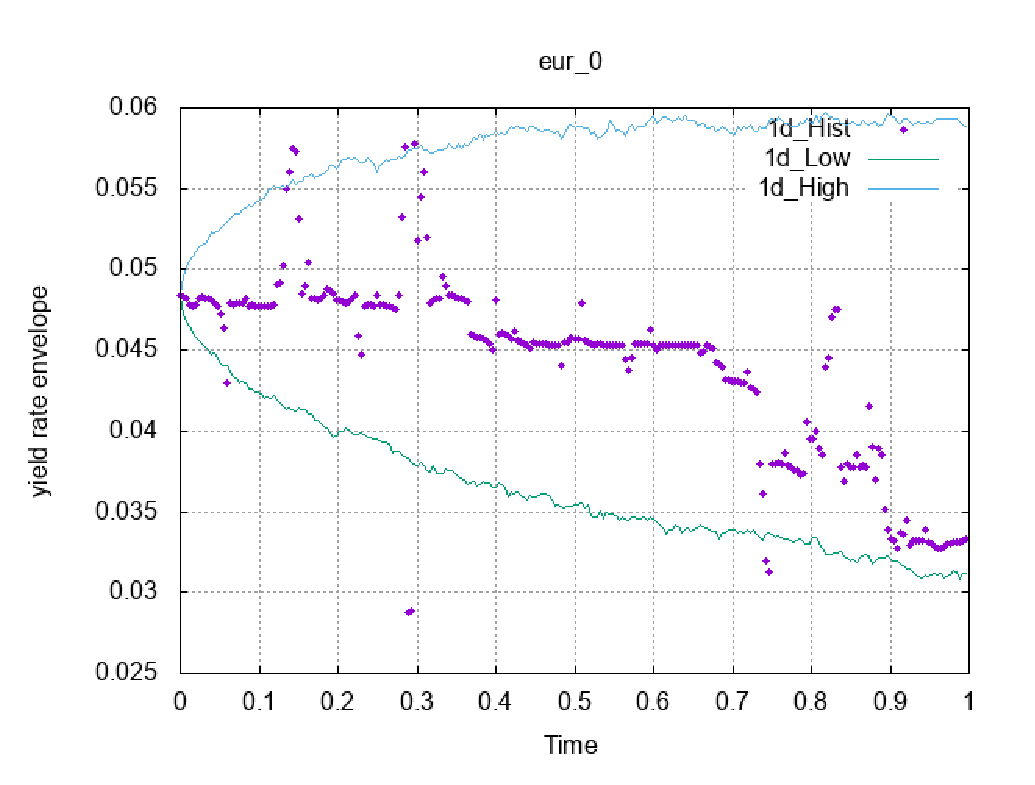
\includegraphics [width=1\textwidth]{blank.eps}
\caption{Excel front end for HJM model calibration}
\label{fr_end}
\end{figure}



\section{Calibration examples} \label{hjm_ex}



\subsection{Single yield curve calibration}

In this section we present results of the model calibration for single yield curve (GBP). The $C^{++}$ application was used with the following input data. \\
Control parameters:

\begin{tabular}{ |l | l | }
\hline
0	&	\text{Starting date for reading data from historical rates files}\\
252	&\text{Number of lines/days to read from historical rates files beginning from starting day} \\
0	&\text{Single curve calibration} \\
252	&\text{Number of days in one year - convention} \\
0.95	&\text{Confidence level} \\
5000	&\text{Number of Monte Carlo scenarios} \\
1	&\text{Penalty weight} \\
gbp\_2001\_2018.in	&\text{File for historical rates in GBP } \\
hjm\_A.in	&\text{File with initial parameter values, and corresponding constraints, for GBP} \\
0.25	&\text{Nelder-Mead iteration step} \\
0.000001	&\text{Terminating limit for the variance of object function values} \\
10	&\text{Convergence check period} \\
300	&\text{Maximal number of object function evaluations} \\
out\_data\_A.csv	&\text{File for GBP output of visualization of calibration results} \\
obj\_fn.csv	&\text{File for object function values versus iterations} \\
report.txt	&\text{Calibration summary output file} \\
1	&\text{Yes for graphical output} \\
1	&\text{Maturities indexed 0, 1 and 7 will be displayed in graphical output} \\
\hline
\end{tabular}
\\


\begin{figure}[H]
\centering
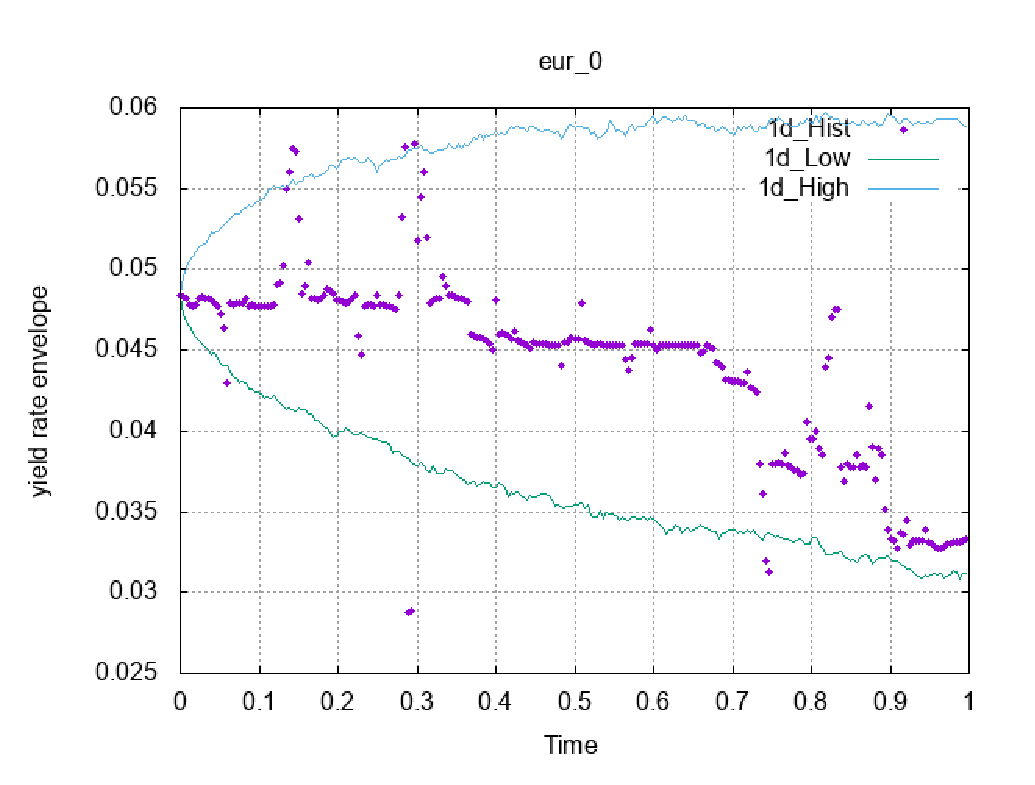
\includegraphics [width=1\textwidth]{blank.eps}
\caption{Object function for calibration of GBP yield curve on market data of 2011}
\label{Q1}
\end{figure}


\begin{figure}[H]
\centering
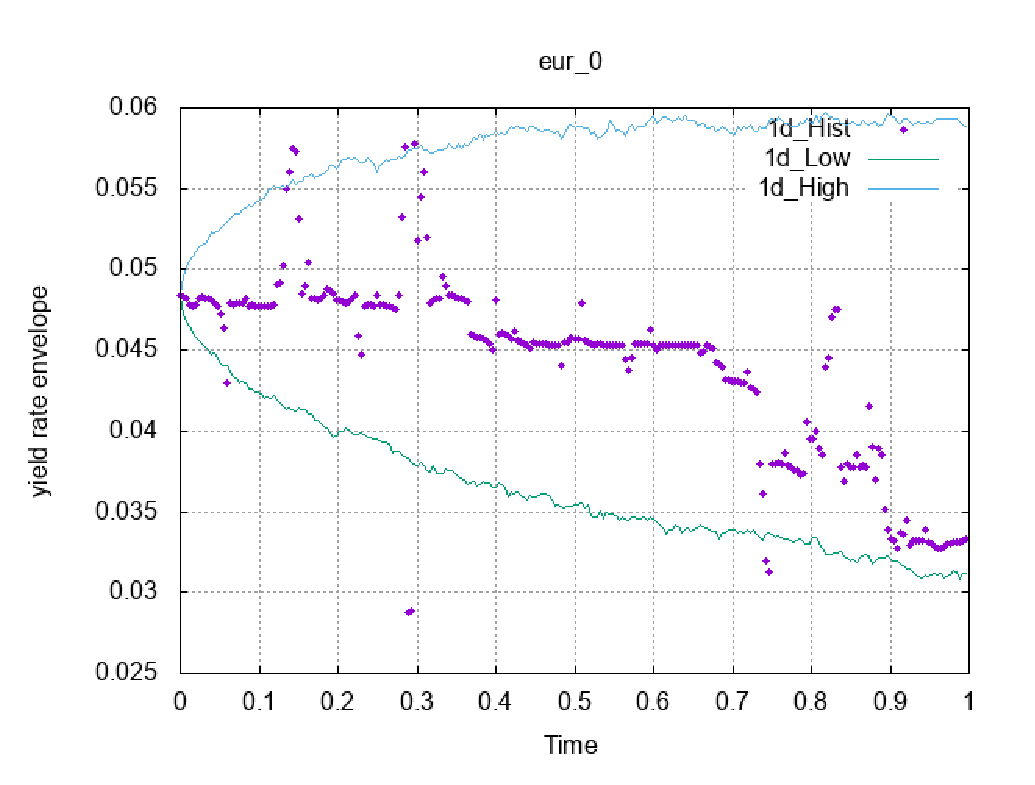
\includegraphics [width=1\textwidth]{blank.eps}
\caption{Simulation of GBP overnight (1 day) rate on optimal HJM parameters. Historical data 2011: dots, upper and lower percentiles of simulated rates: lines}
\label{gbp0}
\end{figure}

\begin{figure}[H]
\centering
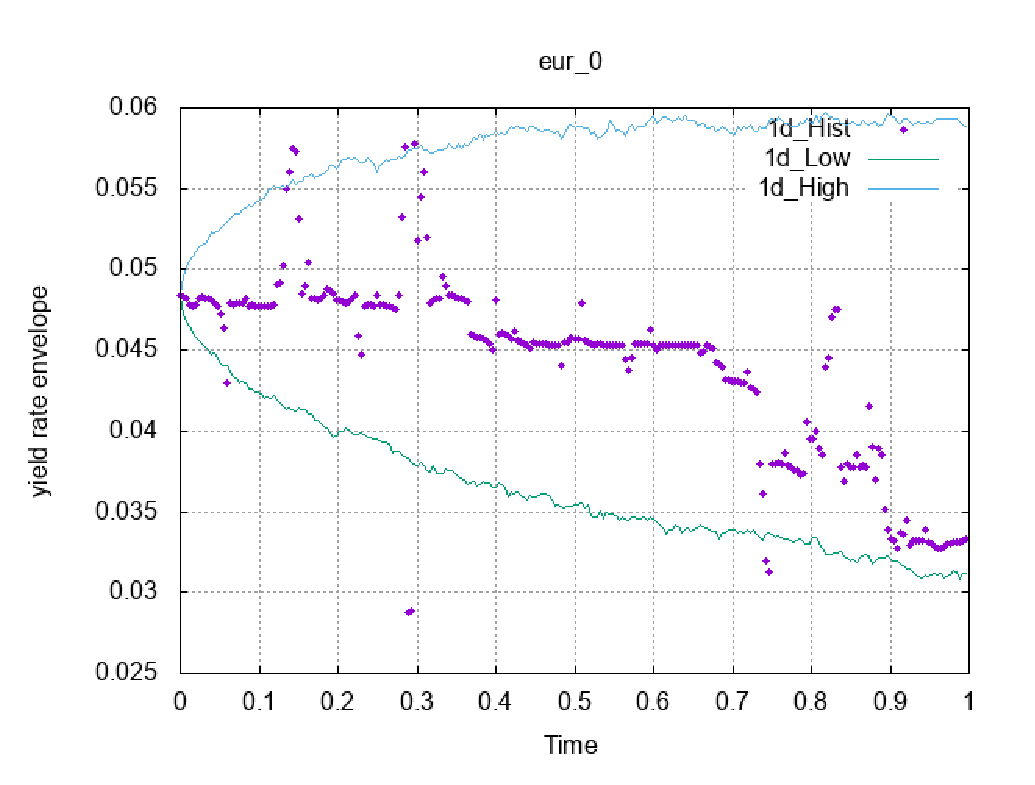
\includegraphics [width=1\textwidth]{blank.eps}
\caption{Simulation of GBP rate (maturity 1 year) on optimal HJM parameters. Historical data 2011: dots, upper and lower percentiles of simulated rates: lines}
\label{gbp2}
\end{figure}


\begin{tcolorbox}

Calibration report:

\begin{verbatim}
Calibration run
Started: 11_December_2018_01_07_54_AM
Data length: 252 days
Days per year: 252
Confidence level: 0.95
Number of Monte-Carlo scenarios: 5000
Penalty weight: 1
Currency A file: gbp_2001_2018.in
Iteration step size: 0.25
Terminating limit: 1e-06
Convergence check period: 10
Number of object function calculations: 300
Constraints A:
   0.8000   1.5000
   0.8000   1.5000
   0.0100   0.1500
   0.0020   0.0500
   0.0010   0.0500
   0.0010   0.0100
  -0.0300   0.2000
  -0.2000   0.1000
  -0.5000   0.1000
   0.0020   0.2500

A starting point:
kappa0	kappa1	kappa2	sigma0	sigma1	sigma2   rho01	 rho02	  rho12	  theta:
1.200  1.200  0.050  0.040  0.002  0.002  -0.200  -0.100  -0.100  0.100

Starting F(x) = -1.19424
err dev at start=1.97033%

A Optimal point:
kappa0	kappa1	kappa2	sigma0	sigma1	sigma2   rho01	 rho02	  rho12	  theta:
1.3185	1.2123	0.0553	0.0330	0.0052	0.0020	 -0.1610	-0.118 	0.001 	0.0165

Return code IFAULT = 2
Resulting  F(x*) = -2.55852
Resulting err dev=1.67629%
Number of iterations = 303
Number of restarts =   0
Ended: 11_December_2018_08_50_19_AM
\end{verbatim}
\end{tcolorbox}

Results presented in this section demonstrate clearly that model parameters obtained in the calibration procedure allow to simulate rates whose percentile envelope (5\% to 95\%) includes historical yield rates.

\subsection{Dual Yield curve Calibration}

In this section we present results of the model calibration for dual yield curves (GBP and EUR). The $C^{++}$ application was used with the following input data. \\
Control parameters:

\begin{tabular}{ |l | l | }
\hline
0	&	\text{Starting date for reading data from historical rates files}\\
252	&\text{Number of lines/days to read from historical rates files starting from starting day} \\
1	&\text{Dual curve calibration} \\
252	&\text{Number of days in year - convention} \\
0.95	&\text{Confidence level} \\
1000	&\text{Number of Monte Carlo scenarios} \\
10	&\text{Penalty weight} \\
gbp\_2001\_2018.in	&\text{File for historical rates in GBP } \\
hjm\_A.in	&\text{File with initial parameter values, and corresponding constraints, for GBP} \\
eur\_2001\_2018.in	&\text{File for historical rates in EUR } \\
hjm\_B.in	&\text{File with initial parameter values, and corresponding constraints, for EUR} \\
1	&\text{Nelder-Mead iteration step} \\
0.000001	&\text{Terminating limit for the variance of object function values} \\
10	&\text{Convergence check period} \\
500	&\text{Maximal number of object function evaluations} \\
out\_data\_A.csv	&\text{File for GBP output of visualization of calibration results} \\
out\_data\_B.csv	&\text{File for EUR output of visualization of calibration results} \\
obj\_fn.csv	&\text{File for object function values versus iterations} \\
report.txt	&\text{Calibration summary output file} \\
1	&\text{Yes for graphical output} \\
1	&\text{Maturities indexed 0, 1 and 7 will be displayed in graphical output} \\
\hline
\end{tabular}
\\


\begin{figure}[H]
\centering
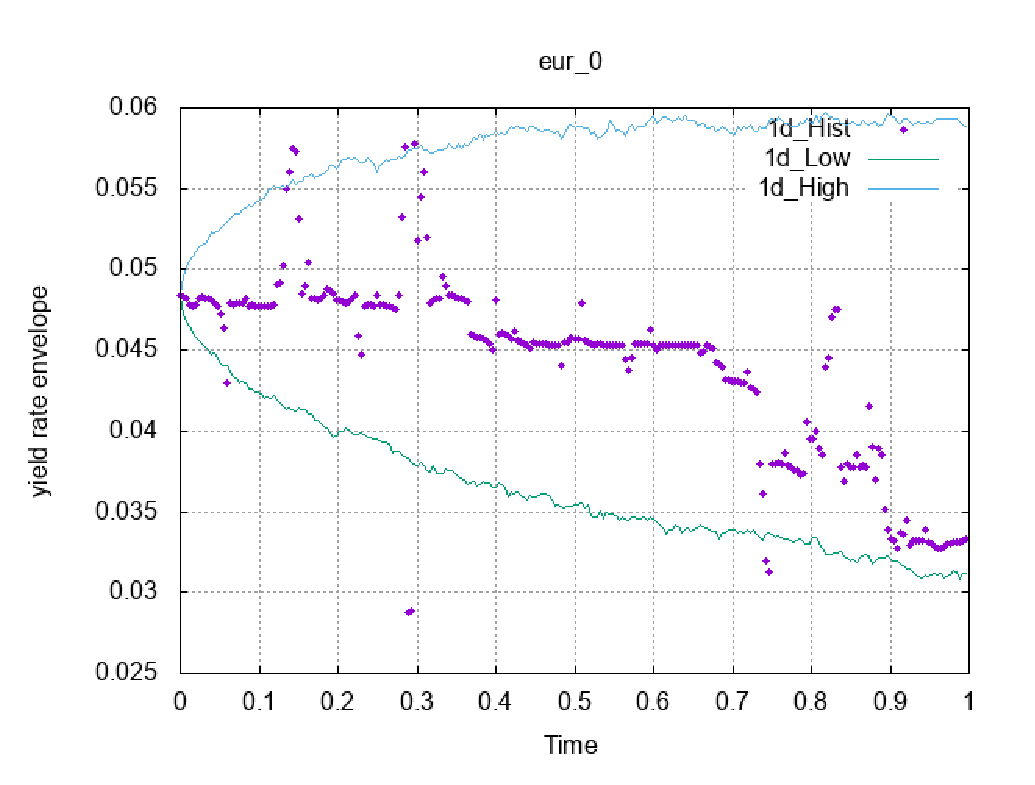
\includegraphics [width=1\textwidth]{blank.eps}
\caption{Object function for calibration of GBP and EUR yield curves on market data of 2011}
\label{Q1d}
\end{figure}


\begin{figure}[H]
\centering
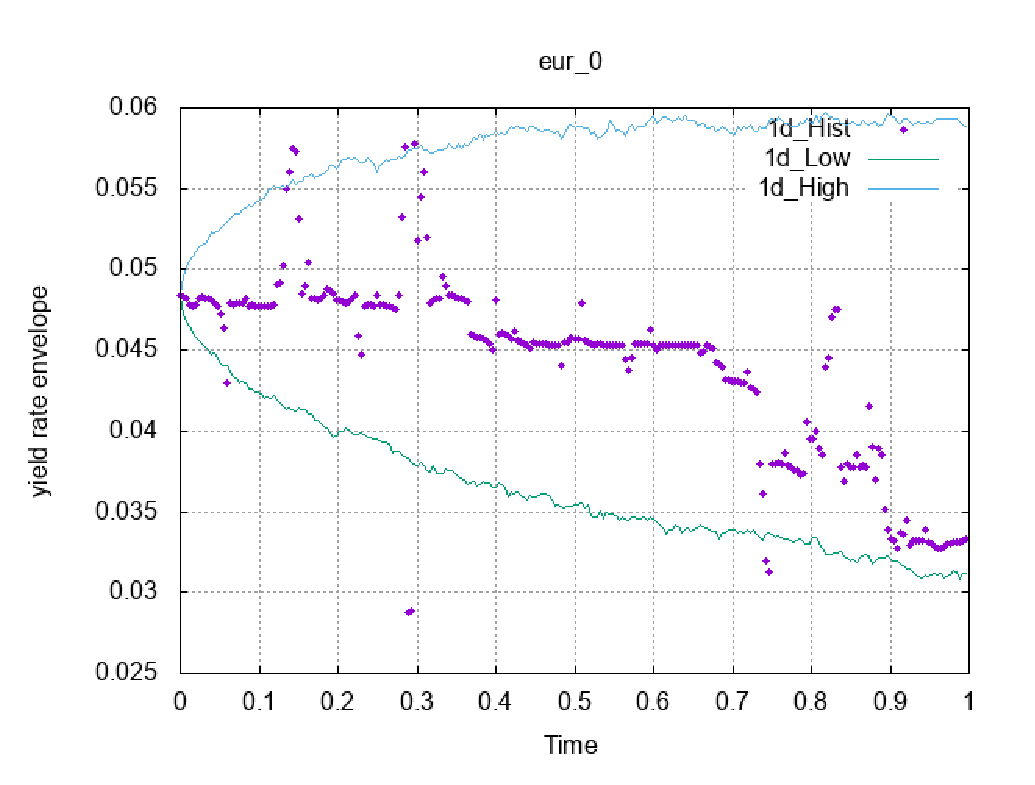
\includegraphics [width=1\textwidth]{blank.eps}
\caption{Simulation of dual GBP/EUR overnight (1 day) rate on optimal HJM parameters. Historical GBP data 2011: dots, upper and lower percentiles of simulated GBP rates: lines}
\label{gbp0d}
\end{figure}

\begin{figure}[H]
\centering
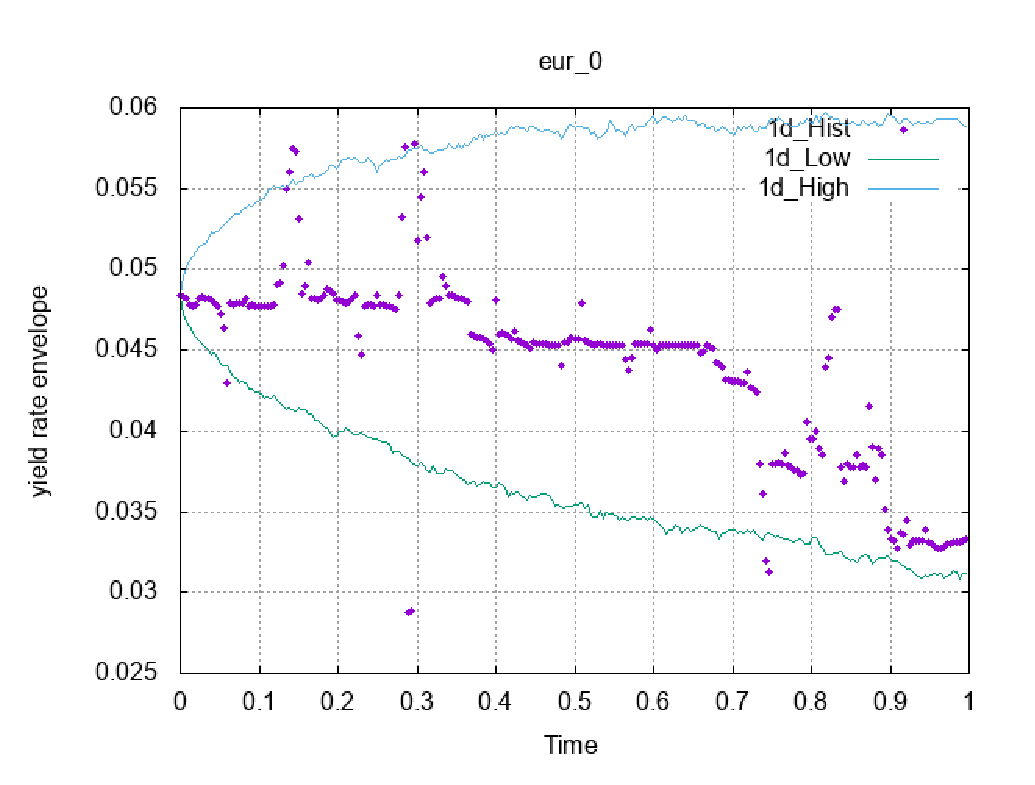
\includegraphics [width=1\textwidth]{blank.eps}
\caption{Simulation of dual GBP/EUR curves (maturity 1 year) rate on optimal HJM parameters. Historical GBP data 2011: dots, upper and lower percentiles of simulated GBP rates: lines}
\label{gbp2d}
\end{figure}

\begin{figure}[H]
\centering
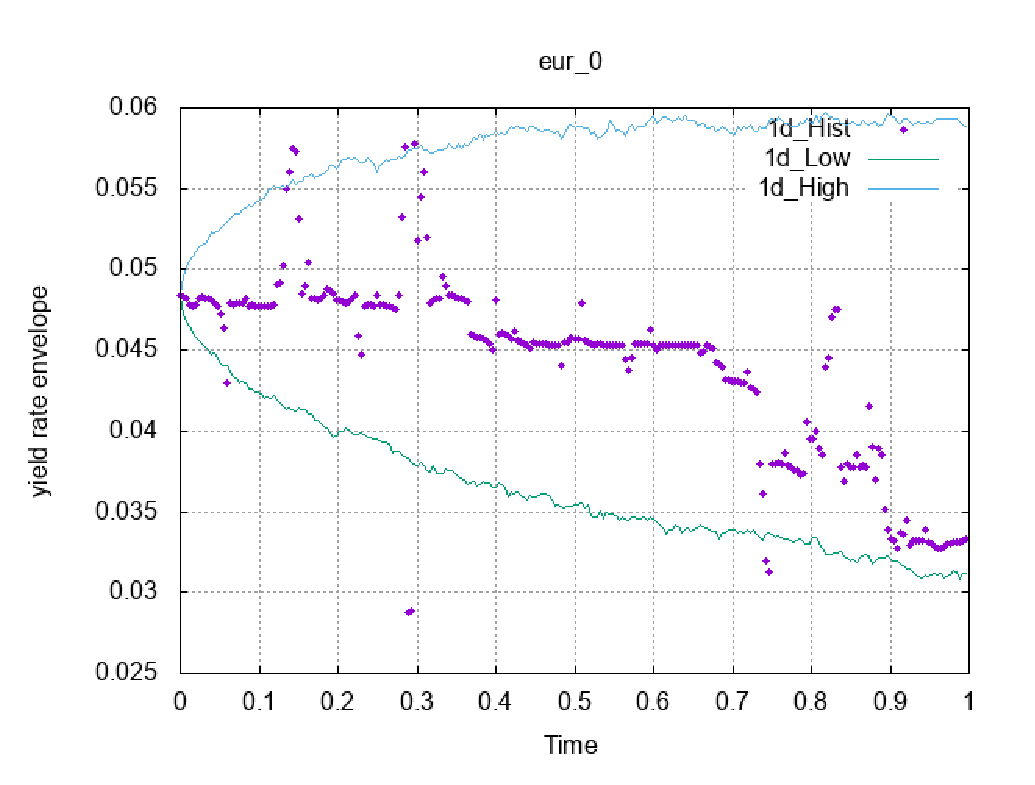
\includegraphics [width=1\textwidth]{blank.eps}
\caption{Simulation of dual GBP/EUR overnight (1 day) rate on optimal HJM parameters. Historical EUR data 2011: dots, upper and lower percentiles of simulated EUR rates: lines}
\label{eur0d}
\end{figure}

\begin{figure}[H]
\centering
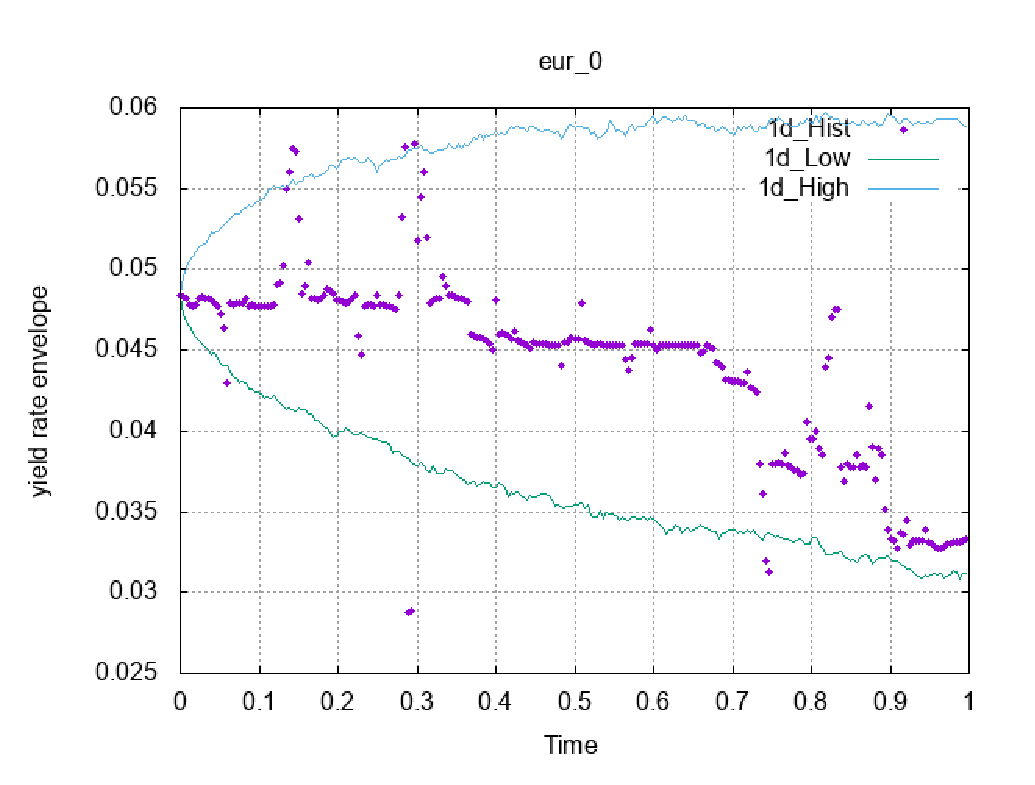
\includegraphics [width=1\textwidth]{blank.eps}
\caption{Simulation of dual GBP/EUR (maturity 1 year) rate on optimal HJM parameters. Historical EUR data 2011: dots, upper and lower percentiles of simulated EUR rates: lines}
\label{eur2d}
\end{figure}

\begin{tcolorbox}

Calibration report for dual curves calibration:

\begin{verbatim}
Started: 20_December_2018_11_16_12_PM
Data length: 252 days,	Days per year: 252,	Confidence level: 0.95
Number of Monte-Carlo scenarios: 1000
Penalty weight: 10
Currency A file: gbp_2001_2018.in,	Currency B file: eur_2001_2018.in
Iteration step size: 1
Terminating limit: 1e-06
Convergence check period: 10
Number of object function calculations: 500
Constraints A			     	Constraints	B
0.100		0.500		     				0.300	1.200
0.100		0.500				     		0.500	1.200
0.030	0.150				     	0.100	0.1500
0.010	0.050				     	0.002	0.010
0.005	0.010				     	0.005	0.030
0.001	0.010				     	0.005	0.020
-0.04	0.100				     		-0.030	0.050
-0.10	0.100				     		-0.140	0.010
-0.50	0.000				     		-0.500	0.000
0.010	0.100				     		-0.300	0.010
						     		     	     	-0.250	0.000
							 	         	     	-0.700	-0.100
A starting point:
kappa0	kappa1	kappa2	sigma0	sigma1	sigma2   rho01	rho02	 rho12	  theta:
0.20   0.20   0.07   0.02   0.008   0.005  -0.02   0.02  -0.20   0.05
B starting point:
kappa0	kappa1	kappa2	sigma0	 sigma1	sigma2   rho01	 rho02	  rho12:
1.00   1.00   0.20   0.007   0.015   0.010  -0.01   -0.07  -0.20 
ksi0	   ksi1	   ksi2:
-0.20  -0.15  -0.50
Starting F(x) = -1.04178
Err dev at start=1.32305%
A Optimal point:
kappa0	kappa1	kappa2	sigma0	sigma1	sigma2 rho01	 rho02	  rho12	 theta:
0.2811	0.2731	0.0768	0.0059	0.0093	0.0090	0.0106	0.0289	-0.2561	0.0110
B Optimal point:
kappa0	kappa1	kappa2	sigma0	sigma1	sigma2 rho01	 rho02	  rho12	 theta:
0.8278	0.9211	0.1481	0.0092	0.0135	0.0179	-0.0052	-0.0863	-0.1929
ksi0	     ksi1   	ksi2:
-0.1551	-0.1395	-0.5218
Return code IFAULT = 2
Resulting  F(x*) = -3.10626
Resulting err dev=1.05731%
  Number of obj fn evaluations = 514
Number of restarts =   0
Ended: 21_December_2018_10_15_32_AM
\end{verbatim}
\end{tcolorbox}

\section{Summary} 


The tri-factor HJM interest rate model calibration algorithm was developed in general case of the dual curve modelling. For the dual-curve model the correlation factors for different currencies were introduced. The calibration algorithm is based on the maximum likelihood criterium: yield rate simulated by Monte-Carlo process fit to the historical data. Minimization of the objective function is based on simplex (Nelder-Mead) method. The $C^{++}$ application for calibration was developed and tested. 

\bibliographystyle{humannat}

\bibliography{refs}		% expects file "refs.bib"


\end{document}


				
	
